\chapter{Research Design}
\label{resdes}
\begin{comment}

\end{comment}

\begin{figure}[h]
	\centering
	\captionsetup{justification=centering}
    \scalebox{.40}{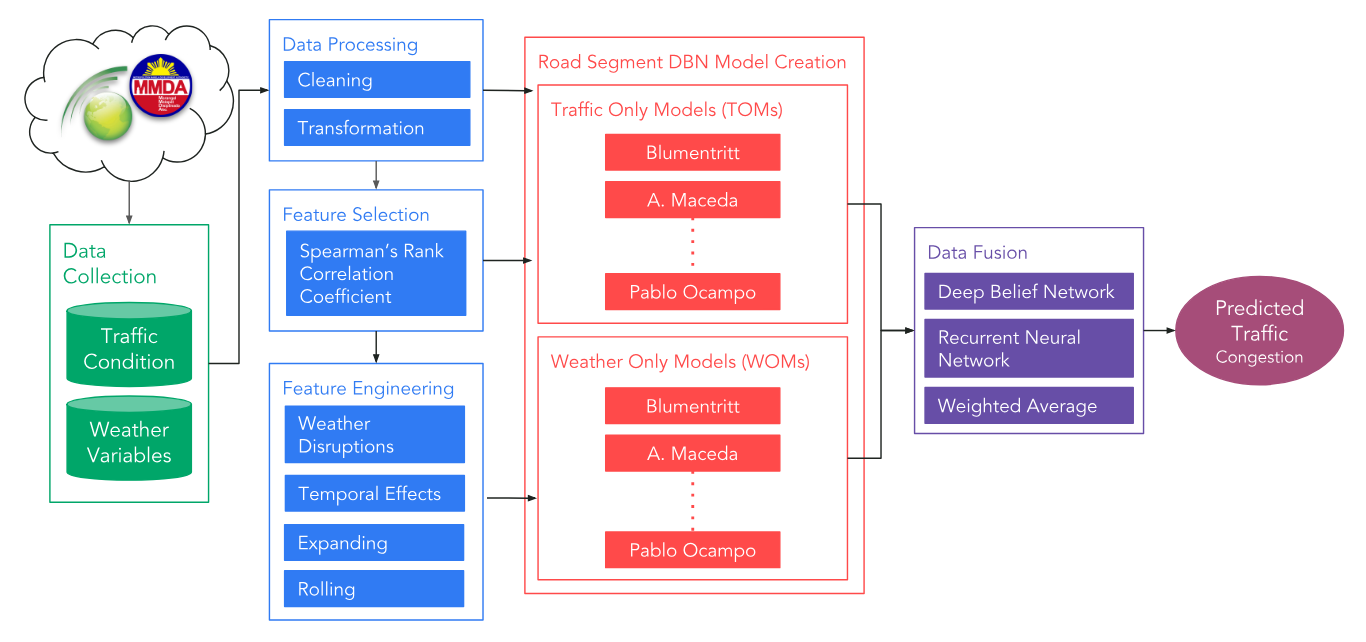
\includegraphics{THESIS_ResearchDesignFinal.png}}
	\caption{Research Framework}
	\label{fig:framework}
\end{figure}



Figure \ref{fig:framework} illustrates the whole framework for the research. First, this research collected historical traffic condition from MMDA and historical weather variables from WWO. These raw data was cleaned and re-sampled to match the time intervals of the data using linear interpolation and was transformed to their normalized values. Both datasets were cross-correlated with each other to analyze and determine significant weather variables. Aside from that, the effects of extreme weather disruptions to traffic were explored. Furthermore, that may neglect the effect of weather on traffic were also explored. From these analyses, features were extracted that would better represent the data for our problem through \textit{feature engineering} using rolling and expanding. 

The final variables and engineered features were fed into the Traffic-Only Models (TOM) and Weather-Only Models (WOM), which were developed in DBN, for 14 roads in Manila. Following the DEI-DEO fusion technique, the predicted traffic congestion for TOM and WOM were fused in a fusion model, in which three methods of fusion was compared. The model was evaluated using RMSE, MAE, and sensitivity analysis. To achieve a high accuracy, the model's parameters were calibrated based from previous experiments. 


\section{Data Collection} \label{rd_datacollection}
There were two datasets collected: traffic and weather. The traffic dataset was obtained from Metro Manila Development Authority (MMDA) traffic monitoring system. The weather dataset was collected from World Weather Online (WWO). Both datasets were collected from May 2015 to October 2015, highlighting the wet season in the Philippines.

\subsection{Traffic Dataset}
There were two limitations found from the traffic dataset. First is that the traffic conditions were only represented as \textit{light} (L), \textit{moderately light} (ML), \textit{moderate} (M), \textit{moderately heavy} (MH), and \textit{heavy} (H). Since this dataset only had five values to classify the traffic condition in a particular road segment, this might cause underfitting in our model since it was used as input for a regression problem. Moreover, it could also contribute to poor correlation as these five values were correlated with continuous weather variable values. To have the traffic conditions be continuous values, they were converted to their equivalent estimated traffic speed provided by the MMDA (see Table \ref{table_traffic_condition}). These speeds are further converted to congestion levels, represented as their reciprocal so that the data would be easier to interpret such that higher value means higher congestion level.

\begin{table}[h]
\centering
\caption{Traffic speed equivalent of traffic conditions}
\label{table_traffic_condition}
\begin{tabular}{|l|r|}
\hline
\textbf{Traffic Condition} & \multicolumn{1}{l|}{\textbf{Equivalent Speed (kph)}} \\ \hline
Light (L)                  & 36 - 60                                             \\ \hline
Moderately Light (ML)                  & 31 - 35                                            \\ \hline
Moderate (M)               & 16 - 30                                             \\ \hline
Moderately Heavy (MH)                  & 11 - 15                                             \\ \hline
Heavy (H)                  & 0 - 10                                              \\ \hline
\end{tabular}
\end{table}


Another limitation was that the traffic dataset contains missing records. Out of 4,749,417 records, there were 522 rows wherein the traffic condition of that road segment in that particular time interval was not recorded, as indicated by \textit{none} (N) condition. Furthermore, having only 4,749,417 records from a sample from 2015, having a 15-minute interval for 142 road segment, meant that 226,263 records or 16 days of data were missing as well. This implied that inconsistencies may occur as the missing data would need to be filled to make the data continuous. To do this, those missing values were replaced through linear interpolation.

Apart from the limitations, there were other factors considered in this study. Since this study is only concerned road segments from Manila, only the road segments under it were used. As a result, 14 out of 142 road segments were only considered: 7 from Roxas Boulevard and 7 from España.



\subsection{Weather Data}
The collected weather dataset from WWO featured a complete hourly reading of the weather variables for Manila. One downside of this dataset, however, was that the weather data generalizes the weather for the whole city. This implied inconsistencies when correlating the traffic condition to the weather variables as the weather at one road is not the same as the weather of another, despite being in the same city.

Additionally, the hourly weather dataset needed to be matched with the 15-minute interval of the traffic dataset. This was done by resampling and linear interpolating the dataset to have a 15-minute time interval.




\section{Data Analysis}
Given these two independent time-series datasets, analyses were performed to better understand the relationship between weather and traffic. This is accomplished by identifying the weather variables that influence traffic. From that, we further explore the effects of extreme weather disruptions, such as typhoons and tropical depressions, to traffic. Furthermore, we also explored traffic trends that may neglect the effect of weather on traffic. From these analyses, we extracted features that would better represent the data for our problem through \textit{feature engineering}. Feature engineering is a process that aims to improve the prediction performance of a model by using domain knowledge to generate features based on the raw data.


\subsection{Weather and Traffic}

\subsubsection{Weather Variables Influencing Traffic}
It is important to understand the relationship between the weather variables and the traffic congestion. To ensure that only the most relevant variables were selected and only those which would best yield an accurate prediction, correlation was performed. Using Spearman's rank correlation coefficient, the traffic speed was correlated with the weather variables. If a weather variable has low correlation with the traffic condition, it would be discarded. Similarly, to reduce redundancy and to properly select only the weather variables that shape traffic condition, weather factors were correlated with each other. If a weather variable has large correlation coefficients in relation with the highest cross-correlation coefficient, it would be discarded since it is redundant.

\subsubsection{Effect of Weather Disruptions of Traffic}
In this study, analysis on the effects of extreme weather disruptions to traffic was performed. In areas like Manila, which has an inadequate drainage system and poor road infrastructure, the build-up of these downpours may cause flood, which may contribute to the traffic of certain areas as the rainfall does not runoff effectively. 

To model these conditions, three factors was considered: the precipitation build-up, the traffic build-up and the delay of the effect. The build-up of the amount of precipitation for the prolonged rain periods was derived. This involves getting the cumulative precipitation amount as time passes by. Meanwhile, for traffic build-up, the growth of traffic congestion level is only considered since the more granular effects of precipitation due to traffic speed being derived from ordinal traffic conditions. Thus, the stability and the decay of traffic were filtered out. Consequently, a comparison of a normal congestion level transition and a congestion level spike was studied. These analyses used Spearman’s correlation. 

\subsection{Feature Engineering of Traffic Trends}
Aside from the effects of weather to traffic, it is also important to analyze the temporal effects in the variations of traffic pattern. In terms of traffic, the holidays and day-of-week affect when and how much people travel to one place to another \shortcite{cools2007investigating}. Because people are on duty during working days, usually from Mondays to Fridays, this implies an increase in demand on transportation when going to their respective organizations. Aside from working days, the time when the majority of people travel, also called peak hour, is also necessary to take into account. 


\subsection{Feature Engineering of Time Series}
Rolling and Expanding features were generated for windows \textit{2, 3, 4, 8, 12, 24, 48}, and \textit{96} for both traffic and weather, where a window represents a 15-minute time interval, for analysis. The statistical features that were generated were the mean, minimum and maximum for both rolling and expanding windows, describing the trend of the given window size $w$ at previous time step $w$.

In order to analyze the relationship between traffic trends, the autocorrelation of traffic was generated, and the cross correlation between the original traffic and the engineered features of rolling and expanding was analyzed. From there, the optimal rolling and expanding windows for both traffic and weather were then identified as additional features for TOM and WOM. 



%TRAFFIC MODEL CREATION
\section{Model Implementation}

\subsection{Prediction Models}
According to the framework in \ref{fig:framework}, two models were implemented using Deep Belief Network (DBN): the Traffic-Only model (TOM), which only considers traffic to predict, and the Weather-Only model (WOM), which only considers weather variables to predict traffic. In this study, the DBN models were run using tensorflow.  There are three layers for both TOM and WOM with 20, 50, and 100 nodes respectively. Epochs for RBM is 5, while epochs for DBN is 150. Learning rate for both DBN and RBM is 1%. 


\subsection{Data Fusion Model}
This study’s framework followed a Decision In-Decision Out (DEI-DEO) fusion technique, in which the predicted traffic congestion from TOM and WOM would be fused together to make a more decisive prediction. This study also compared Feature In-Decision Out (FEI-DEO) fusion technique, in which features from both the traffic and weather dataset would be fused together first before generating the predicted traffic congestion, to DEI-DEO framework. Three methods of data fusion were tested for the fusion step of the whole model: Weighted Average, Artificial Neural Network, and Deep Belief Network. 

%WEIGHTED AVERAGE
\subsubsection{Weighted Average} 
The weighted average data fusion method accepts a combined dataset of all three factors and outputs a more consistent dataset to be fed into a prediction model. In this method, the traffic and weather dataset were merged into one dataset. Each input in the resulting dataset was multiplied with its corresponding weight. Each weight was assigned based on the importance of the variable considered while keeping in mind that the sum of the weights should be equal to 1. The resulting dataset was then be summed up to get the output mean. This was to serve as an input to the distribution method to be applied to the dataset. The resulting consistent dataset were then fed to the prediction models.

%NEURAL NETWORK
\subsubsection{Neural Network}
The fusion model was also developed in two neural networks: Recurrent Neural Network (RNN) and Deep Belief Network (DBN) for the two fusion techniques.

In FEI-DEO, the traffic congestion and weather variables were fused into one dataset, which was then fed into the network. The network will be trained to predict the traffic condition affected by the information from the weather with flood from $t$ to $t-8$. The training of the network will continuously adjust weights and biases from comparing the generated output with the actual traffic condition. In merging the features, the relationship of the weather variables collected from the correlation analysis will be considered in adjusting the weights and biases. 

The RNN for FEI-DEO fusion will only have 1 input layer, 1 hidden layer, and 1 output layer. The number of units for the hidden layer of the RNN will be determined through trial and testing starting from 5 to 100 units. The network graph for RNN for FEI-DEO fusion is illustrated in \figref{fig:feideo_ann}. 
\begin{figure}[h]
	\centering
	\captionsetup{justification=centering}
	\scalebox{.6}{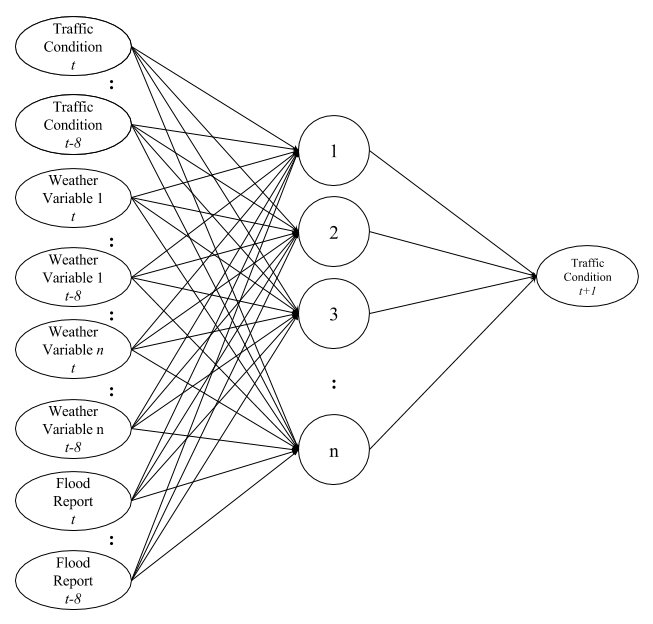
\includegraphics{feideo_ann.png}}
	\caption{Structure of the FEI-DEO Fusion Model using ANN}
	\label{fig:feideo_ann}
\end{figure}

The DBN for FEI-DEO fusion have 1 input layer, 3 hidden layers, and 1 output layer. This epochs of DBN was 150 and 5 epochs for RBM. The units for each hidden layer are 20, 50, and 100 respectively. The learning rate for this fusion is 0.01 for both DBN and RBM. The network graph for DBN for FEI-DEO fusion is illustrated in \ref{fig:feideo_dbn}. 

\begin{figure}[h]
	\centering
	\captionsetup{justification=centering}
	\scalebox{.6}{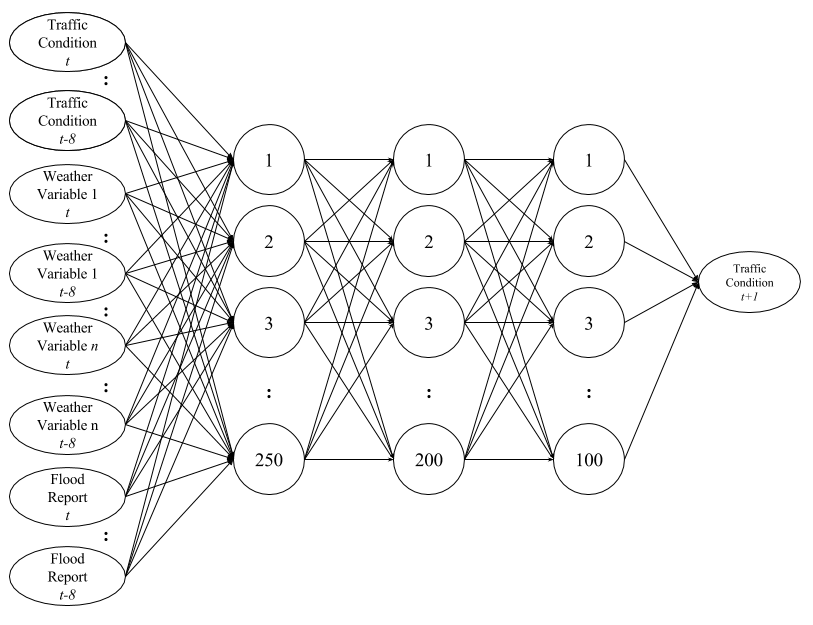
\includegraphics{feideo_dbn.png}}
	\caption{Structure of the FEI-DEO Fusion Model using DBN}
	\label{fig:feideo_dbn}
\end{figure}

In DEI-DEO, the inputs will first be fed into the two Prediction Model. The predicted traffic condition generated by these Prediction Models will be fed into the fusion model. The network will be trained to predict the traffic condition $t+1$ in the future through a backpropagation by comparing the generated traffic condition prediction to the expected prediction, and adjusting the weights and biases of units and layers to fuse the two decisions to arrive to a prediction close to the expected. The input layer will have the predicted traffic condition of Prediction Model 1 and Prediction Model 2. These decisions will be fed into the hidden layer of the network, and into the output layer for the final predicted traffic condition of $t+1$ in the future. 

The Artificial Neural Network for DEI-DEO fusion will only have 1 input layer, 1 hidden layer, and 1 output layer. The number of units for the hidden layer of the Artificial Neural Network will be determined through trial and testing starting from 5 to 100 units. The network graph for ANN for DEI-DEO fusion is illustrated in \figref{fig:deideo_ann}. 

The Deep Belief Network for DEI-DEO fusion will only have 1 input layer, 3 hidden layers, and 1 output layer. The DBN for fusion will be similar with the network for Prediction in terms of layer and unit number except for the input layer that will consist of the decisions from Prediction Model 1 and Prediction Model 2. The network graph for DBN for DEI-DEO fusion is illustrated in \figref{fig:deideo_dbn}.

\begin{figure}[h]
	\centering
	\captionsetup{justification=centering}
	\scalebox{.6}{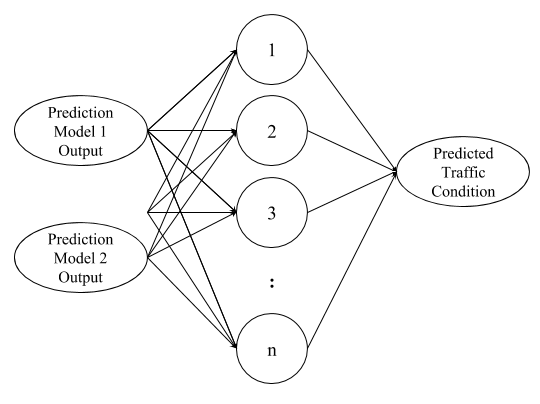
\includegraphics{deideo_ann.png}}
	\caption{Structure of the DEI-DEO Fusion Model using ANN}
	\label{fig:deideo_ann}
\end{figure}

\begin{figure}[h]
	\centering
	\captionsetup{justification=centering}
	\scalebox{.6}{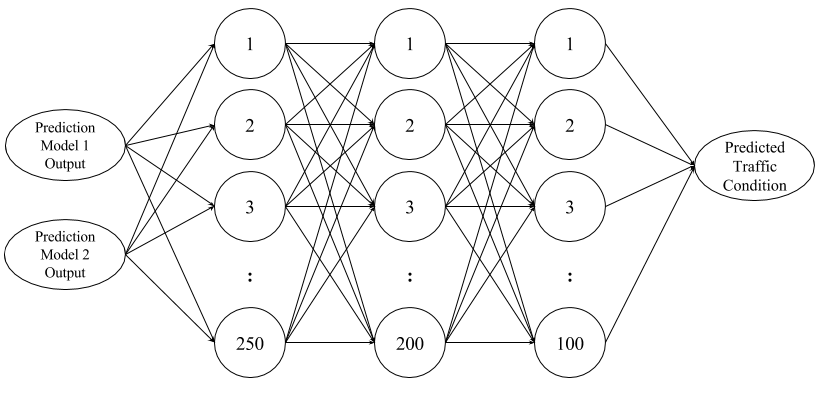
\includegraphics{deideo_dbn.png}}
	\caption{Structure of the DEI-DEO Fusion Model using DBN}
	\label{fig:deideo_dbn}
\end{figure}
\section{Evaluation}
%[Comparing of Performances]
The performance of the prediction models was evaluated using RMSE and MAPE. Additionally, the performance of the fusion model fusing in the feature level (FEI-DEO) and in the decision level (DEI-DEO) was compared and evaluated. Following DEI-DEO framework, the performances of TOM and WOM were evaluated first to see the accuracy of the prediction before fusing. The performance of the three fusion methods (weighted average, RNN, and DBN) were compared and evaluated to see the accuracy of the final prediction. Following FEI-DEO framework, the fusion model using the three fusion methods were compared to the DEI-DEO framework results. 

The overall comparison of the prediction of TOM, wherein traffic congestion is predicted using traffic data only, and the prediction of the final decision of the main model framework, wherein traffic congestion is predicted using both traffic and weather data, were evaluated in this study. 


%Galing pa to before revisions :) 
% how
The sensitivity of the model will also be evaluated and analyzed. Parameters of the networks will be tinkered and experimented to see the sensitivity of the model. The resulting weather variables from the correlation analysis will serve as input to the model, with varying adjustments. For example, if one of the resulting weather variables is precipitation (rainfall), we will test how our model will predict traffic when we input a range of input for rainfall $\{0mm, 2mm, …, 20mm\}$. Hyperparameters will also be calibrated such as the learning rate, epochs, the number of units in the hidden layers for the improvement of the network.


%The model will have two predictors, one for predicting traffic which will be referred to as the Prediction Model 1, and the other for predicting weather which will be referred to as the Prediction Model 2. % 
The model will have two predictors, both for predicting traffic but varying inputs. Both predictors will use Deep Belief Network for its prediction algorithm. For the input of the models, historical traffic condition will be fed into the Prediction Model 1, and the values  of the historical significant weather variables and flood reports will be fed into the Prediction Model 2. Both prediction models will have an output of predicted traffic condition for all 46 road segments. The framework of the model will follow the Decision In - Decision Out (DEI-DEO) data fusion where the two predictions will be fused together using data fusion techniques. The model will also be tested with the Feature In - Decision Out (FEI-DEO) will be compared to the chosen fusion method for analysis.

The rest of this section is organized as follows: Section 4.3.1 discusses the implementation of Prediction Model 1 and 2 using DBN. Section 4.3.2 discusses the implementation of the the data fusion techniques using ANN, DBN, and Weighted Average. 

%PREDICTION MODEL
\subsection{Prediction Model}
Deep Belief Network (DBN) is made up of stacks of Restricted Boltzmann Machines. The training for DBN consists of two phases: pre-training and fine-tuning. In pre-training, each RBM is trained individually, and weights and biases of layers are fixed. In fine-tuning, the weights and biases of the whole network will be updated via back propagation using labeled input data. 

Figure \ref{fig:dbntraining} shows the process of how the Prediction Models using DBN will be trained for prediction. The training process consists of three stages. In the first stage, the stacks of RBM (SRBM) within the network will be trained individually. At the end of this stage, the weights and biases of the whole DBN are initialized. In the second stage, the DBN will fine tune the initialized weights and biases using backpropagation algorithm. The network after stage 2 will be the trained and enhanced DBN. In the third stage, the network will predict the future traffic condition using a testing dataset.

\begin{figure}[h]
	\centering
	\captionsetup{justification=centering}
	\scalebox{.8}{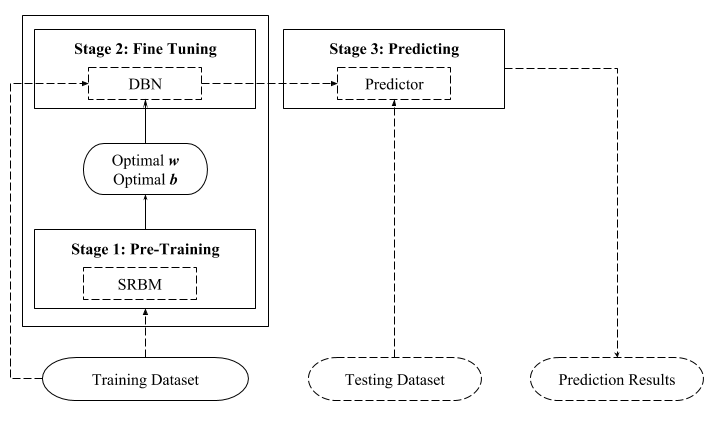
\includegraphics{dbntraining.png}}
	\caption{Structure of DBN Training Process}
	\label{fig:dbntraining}
\end{figure}

For the pre-training phase, the SRBM will perform a number of forward and backward passes until the reconstructed data is close to the original input. The process of backward and forward passes is performed using the equations \ref{eq:4} and \ref{eq:5} to compute for the conditional probability of the hidden unit $h_j$ and visible unit $v_i$, respectively. 

%Fine Tuning
For the fine-tuning phase, the loss function and activation function is defined.
The loss function for the softmax layer to improve the learning rate will use the cross-entropy equation between the visible and hidden units. The cross-entropy function is defined as 
\begin{equation}
C = -\frac{1}{n}\sum_x [y ln a + (1 - y) ln (1-a)]
\end{equation}
\noindent where $n$ is the size of the training data, $x$ is the training input, $y$ is the desired output, and $a$ is the unit’s output. 
For the activation function in the fine-tuning phase, the sigmoid of the feature element-wise will be used. The sigmoid function is defined as 
\begin{equation}
f(x) = \frac{1}{1+e ^{-x}}
\end{equation}

The DBN for the prediction model will have three hidden layers (four RBMs) with 250 units in the first hidden layer, 200 units in the second, and 100 in the third. The learning rate for the RBM will be 0.01. There will be a max of 100 epochs. The batch size of the network will be 10. The number of Gibbs Sampling steps will be 8. 

The input layer for Prediction Model 1 will accept the sequential traffic condition starting from $t-8$ which is the time 120 minutes before the prediction until $t$ which is the time 15 minutes before the prediction. The input layer will have time series data of the traffic condition from $t$ to $t-8$ in the past, time lag being 8. To train the model to predict the traffic condition of all 46 road segments, each road segment will have their own prediction model. The model of road segments that display almost similar patterns of traffic of given time in traffic will be merged into one model. 
The input layer for Prediction Model 2 will accept the sequential data for significant weather variables and flood reports starting from $t-8$ which is the time 120 minutes before the prediction until $t$ which is the time 15 minutes before the prediction.
The output layer of the two Prediction Models will only consist of one unit that will contain the predicted traffic condition 15 minutes ahead of $t$ of any road segment. The DBN for the Prediction Model is illustrated in \figref{fig:dbnpredictor}.

\begin{figure}[ht]
	\centering
	\captionsetup{justification=centering}
	\scalebox{.7}{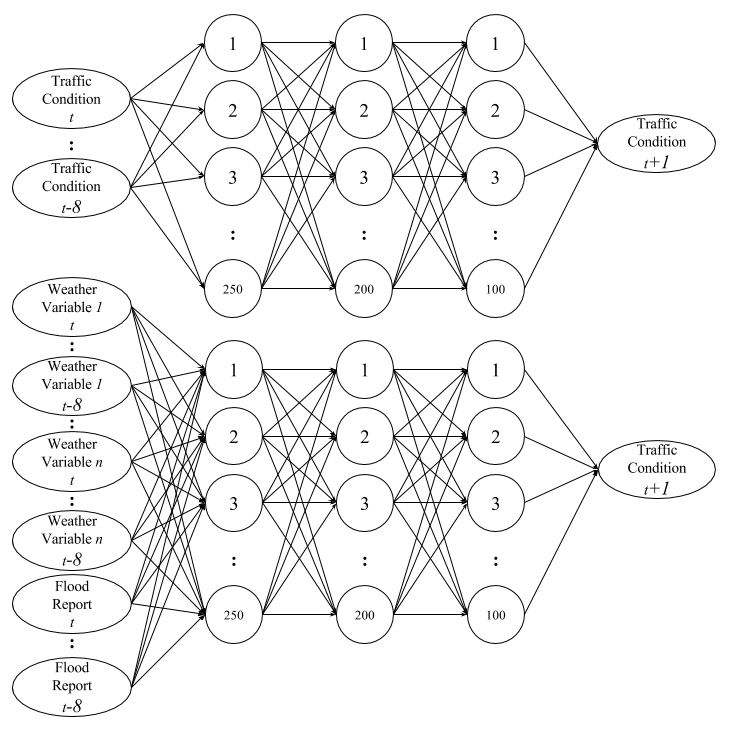
\includegraphics{dbnpredictor.png}}
	\caption{Network Graph of DBN for Prediction Model 1 and 2}
	\label{fig:dbnpredictor}
\end{figure}

\subsection{Fusion Model}
Two fusion schemes will be tested and compared which are the FEI-DEO and DEI-DEO. FEI-DEO will fuse the features of the traffic, weather, and flood. The fused feature will then be fed into a predictor to generate the final predicted traffic condition. In DEI-DEO, the features of traffic, weather, and flood will be predicted separately through Prediction Models. The two predictions will be fused into one final predicted traffic condition. \figref{fig:feideo_vs_deideo} illustrates the structure of the model following the FEI-DEO and DEI-DEO.
Three  methods of data fusion will be tested for the fusion step of the whole model: Weighted Average, Artificial Neural Network, and Deep Belief Network. 

\begin{figure}[h]
	\centering
	\captionsetup{justification=centering}
	\scalebox{.7}{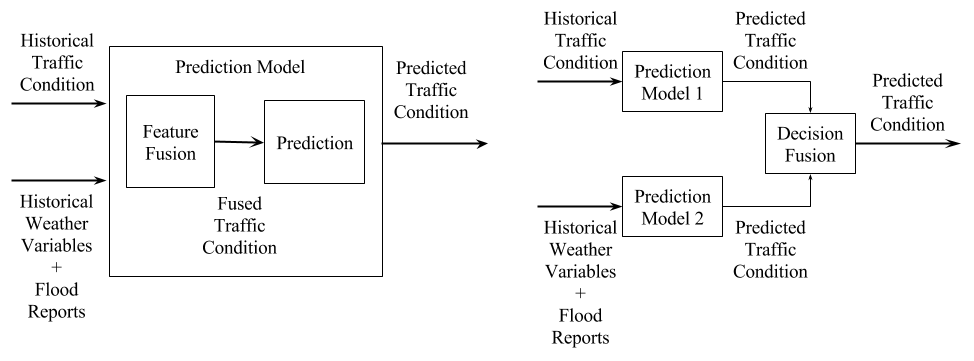
\includegraphics{feideo_vs_deideo.png}}
	\caption{Structure of the model using FEI-DEO (on the left), and DEI-DEO (on the right)}
	\label{fig:feideo_vs_deideo}
\end{figure}

%WEIGHTED AVERAGE
\subsubsection{Weighted Average} 
One fusion method that will be tested is the weighted average method. This method accepts a combined dataset of all three factors and outputs a more consistent dataset to be fed into a prediction model.

In this method, the traffic condition, weather variables, and flood reports will be combined into one data set. Each input in the resulting data set will then be multiplied with its corresponding weight. Each weight is assigned based on the importance of the variable considered while keeping in mind that the sum of the weights should be equal to 1. 

The resulting set would then be summed up to get the output mean. This will then serve as an input to the distribution method to be applied to the dataset. The resulting consistent dataset will then be fed to the prediction model.

%NEURAL NETWORK
\subsubsection{Neural Network}
The fusion model will be also developed in two networks: Artificial Neural Network (ANN) and Deep Belief Network (DBN) in two fusion levels: FEI-DEO and DEI-DEO. 

In FEI-DEO, the weather variables, flood reports and traffic condition will be fused into one dataset. This dataset will be fed into the neural network. The network will be trained to predict the traffic condition affected by the information from the weather with flood from $t$ to $t-8$. The training of the network will continuously adjust weights and biases from comparing the generated output with the actual traffic condition. In merging the features, the relationship of the weather variables collected from the correlation analysis will be considered in adjusting the weights and biases. 

The Artificial Neural Network for FEI-DEO fusion will only have 1 input layer, 1 hidden layer, and 1 output layer. The number of units for the hidden layer of the Artificial Neural Network will be determined through trial and testing starting from 5 to 100 units. The network graph for ANN for FEI-DEO fusion is illustrated in \figref{fig:feideo_ann}. 
\begin{figure}[h]
	\centering
	\captionsetup{justification=centering}
	\scalebox{.6}{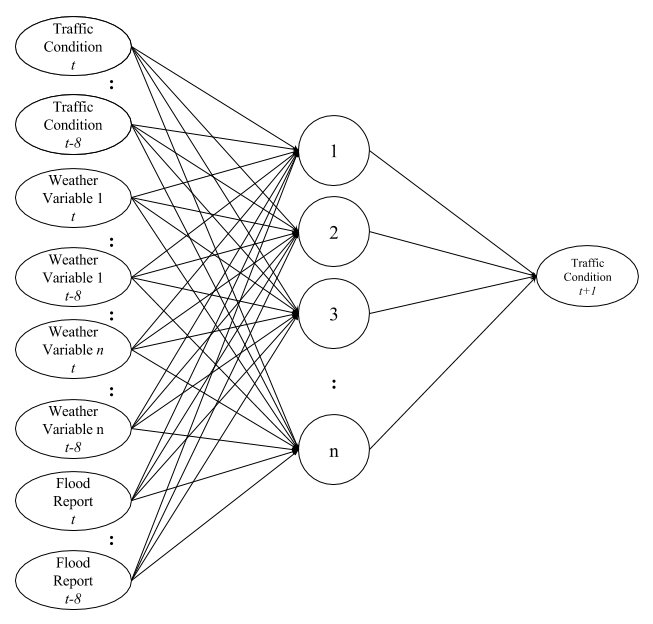
\includegraphics{feideo_ann.png}}
	\caption{Structure of the FEI-DEO Fusion Model using ANN}
	\label{fig:feideo_ann}
\end{figure}

The Deep Belief Network for FEI-DEO fusion will only have 1 input layer, 3 hidden layers, and 1 output layer. The DBN for fusion will be similar with the network for Prediction except for the input layer such that the units in the first hidden layer will be 250 units, the units in the second hidden layer will be 200 units and the units in the third hidden layer will be 100 units. The network graph for DBN for FEI-DEO fusion is illustrated in \ref{fig:feideo_dbn}. 

\begin{figure}[h]
	\centering
	\captionsetup{justification=centering}
	\scalebox{.6}{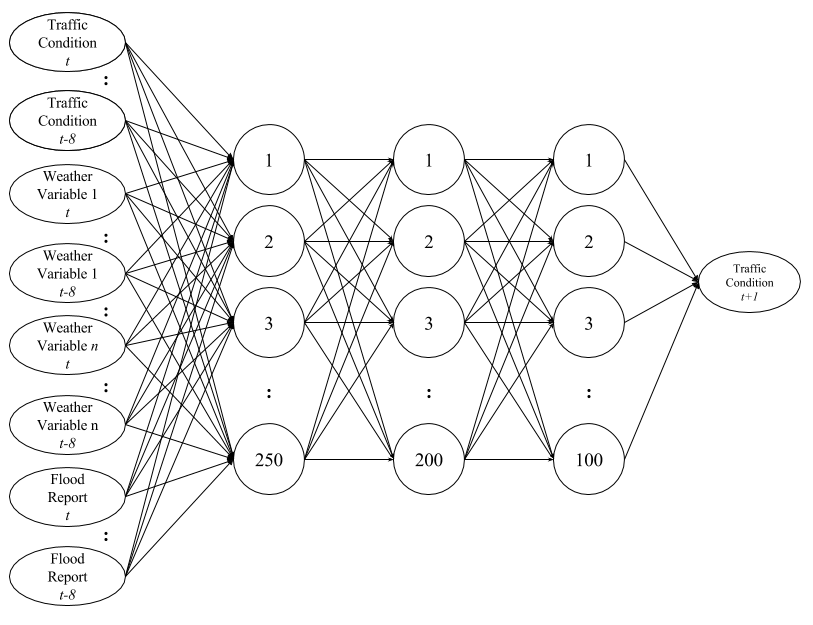
\includegraphics{feideo_dbn.png}}
	\caption{Structure of the FEI-DEO Fusion Model using DBN}
	\label{fig:feideo_dbn}
\end{figure}

In DEI-DEO, the inputs will first be fed into the two Prediction Model. The predicted traffic condition generated by these Prediction Models will be fed into the fusion model. The network will be trained to predict the traffic condition $t+1$ in the future through a backpropagation by comparing the generated traffic condition prediction to the expected prediction, and adjusting the weights and biases of units and layers to fuse the two decisions to arrive to a prediction close to the expected. The input layer will have the predicted traffic condition of Prediction Model 1 and Prediction Model 2. These decisions will be fed into the hidden layer of the network, and into the output layer for the final predicted traffic condition of $t+1$ in the future. 

The Artificial Neural Network for DEI-DEO fusion will only have 1 input layer, 1 hidden layer, and 1 output layer. The number of units for the hidden layer of the Artificial Neural Network will be determined through trial and testing starting from 5 to 100 units. The network graph for ANN for DEI-DEO fusion is illustrated in \figref{fig:deideo_ann}. 

The Deep Belief Network for DEI-DEO fusion will only have 1 input layer, 3 hidden layers, and 1 output layer. The DBN for fusion will be similar with the network for Prediction in terms of layer and unit number except for the input layer that will consist of the decisions from Prediction Model 1 and Prediction Model 2. The network graph for DBN for DEI-DEO fusion is illustrated in \figref{fig:deideo_dbn}.

\begin{figure}[h]
	\centering
	\captionsetup{justification=centering}
	\scalebox{.6}{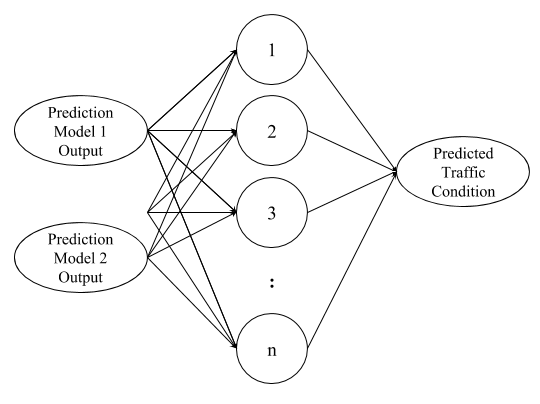
\includegraphics{deideo_ann.png}}
	\caption{Structure of the DEI-DEO Fusion Model using ANN}
	\label{fig:deideo_ann}
\end{figure}

\begin{figure}[h]
	\centering
	\captionsetup{justification=centering}
	\scalebox{.6}{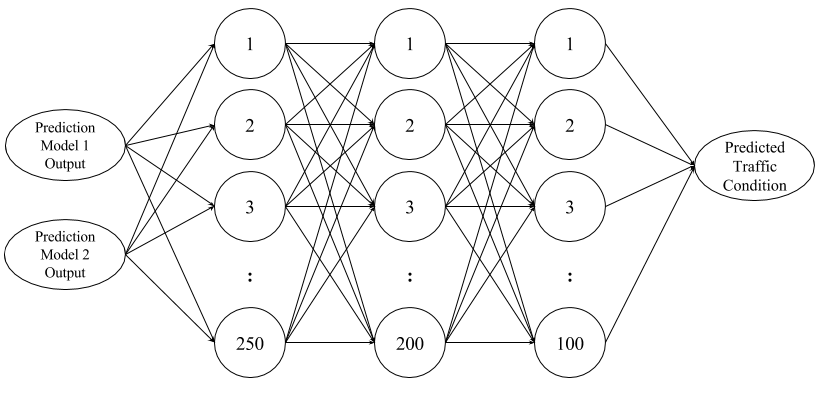
\includegraphics{deideo_dbn.png}}
	\caption{Structure of the DEI-DEO Fusion Model using DBN}
	\label{fig:deideo_dbn}
\end{figure}



%TRAINING
\section{Training}
There will be two types of datasets that will be prepared for the research: the Training dataset and the Testing dataset. The Training dataset will be used during the pre-training and fine-tuning of the model. In the fine-tuning phase of the training of the model, the training dataset will be labeled with the expected output so as to verify and adjust the weights and biases back from the pre-training. The labels will consist of the expected traffic condition given the input data. All data fed into the network are already be normalized. 

%[INSERT TRAINING DATA and TESTING DATA SET FOR PREDICTION MODEL 1]
For the training dataset for Prediction Model 1, two years of historical traffic conditions of 46 road segments from January 2015 to December 2016 will be used, which consists of the dates with 15-minute time intervals, roads, segments, and traffic condition for both northbound and southbound. For the testing dataset, the traffic condition of 46 road segments for the year of 2017 from January to December will be used, which consists of the dates with 15-minute time intervals, roads, segments, and forecasted traffic condition for both northbound and southbound. In this dataset, the forecasted traffic condition will be empty at first, and will be generated by the network. 

%[INSERT TRAINING DATA and TESTING DATA SET FOR PREDICTION MODEL 2]
For the training dataset for Prediction Model 2, two years of historical weather and flood data from January 2015 to December 2016, which consists of the date with 15-minute time intervals, and significant weather variables (e.g. temperature, precipitation, weather condition, etc.) identified from cross-correlating with traffic condition, and flood reports. The testing dataset for Prediction Model 2 is same with Prediction Model 1. 

%[INSERT TRAINING DATA and TESTING DATA SET FOR FUSION MODEL]
For feature-level neural network fusion model, the training dataset is the concatenated datasets of historical traffic condition, historical weather variables, and flood data from the year of January 2015 to December 2016. The concatenated dataset consists of the date with 15-minute time intervals, historical traffic condition, significant historical weather variables, and flood reports. For decision-level neural network fusion model, the training dataset consists of two years of traffic condition predicted by both Prediction Models from the year of January 2015 to December 2016. The dataset consists of the date with 15-minute time intervals and the predicted traffic condition from Prediction Model 1 and Prediction Model 2 for both northbound and southbound. The testing dataset for the neural network-based fusion in feature and decision levels is the same with Prediction Model 1 and 2. 

%[INSERT TRAINING DATA and TESTING DATA SET FOR WHOLE MODEL]
For the whole research, the model will be tested using the testing dataset used for Prediction Model 1 and 2. The accuracy of the final prediction will be tested by predicting the traffic condition of all 46 road segments for the year of 2017 from January to December.
